\documentclass{whutmod}
\usepackage[linesnumbered,ruled,lined]{algorithm2e}
\bibliographystyle{unsrt}
\team{10}
\membera{刘子川}
\joba{编程}
\memberb{程宇}
\jobb{建模}
\memberc{祁成}
\jobc{写作}
\hypersetup{
	colorlinks=true,
	linkcolor=black,citecolor=black
}

\newcommand{\udots}{\mathinner{\mskip1mu\raise1pt\vbox{\kern7pt\hbox{.}}  
		\mskip2mu\raise4pt\hbox{.}\mskip2mu\raise7pt\hbox{.}\mskip1mu}} 

\newcommand{\upcite}[1]{\textsuperscript{\cite{#1}}}
%%%%%%%%%%%%%%%%%%%%%%%%%%%%%%%%%题目%%%%%%%%%%%%%%%%%%%%%%%%%%%%%%%%%%%%
\title{基于卷积自编码的指纹编码与k聚类模型}
\tihao{1} 

\begin{document}

	\maketitle
	\thispagestyle{empty}
%%%%%%%%%%%%%%%%%%%%%%%%%%%%%%%%%摘要%%%%%%%%%%%%%%%%%%%%%%%%%%%%%%%%%%%%
	\begin{abstract}
		控制高压油管的压力变化对减小燃油量偏差,提高发动机工作效率具有重要意义。本文建立了基于质量守恒定理的微分方程稳压模型,采用二分法、试探法以及自适应权重的蝙蝠算法对模型进行求解。
		//
	
		
		针对在小样本条件下难以有效提取指纹特征的问题,设计了一种\textbf{卷积自编码网络}的个体细微特征提取算法。首先将预处理后的图像信号用\textbf{卷积核}转化到高维特征空间,然后利用大量无标签的指纹高维样本训练卷积\textbf{自编码器}网络。在此基础上,通过损失函数\textbf{KL散度}对原始图像和解码后图像\textbf{无监督学习},编码出最佳线性空间特征。经训练提取的指纹特征损失率仅占\textbf{0.04\%},具有精校的还原程度。
		
		
		针对问题二,建立基于质量守恒定律的泵-管-嘴系统动态稳压模型,将燃油进入和喷出的过程动态化处理。考虑柱塞和针阀升程的动态变动,建立喷油嘴流量方程和质量守恒方程。为提高角速度求解精度,以凸轮转动角度为固定步长,转动时间变动步长,采用试探法粗略搜索与二分法精细搜索的方法求解,求得凸轮最优转动角速度\textbf{0.0283rad/ms(转速270.382转/分钟)},并得到该角速度下高压油管的密度、压力周期性变化图。对求解结果进行误差分析与灵敏度分析,考察柱塞腔残余容积变动对高压油管压力稳态的影响。
		
		针对问题三,对于增加一个喷油嘴的情况,改变质量守恒方程并沿用问题二的模型调整供、喷油策略,得到最优凸轮转动角速度为\textbf{0.0522rad/ms(498.726转/分钟)};对于既增加喷油嘴又增加减压阀的情况,建立基于自适应权重的蝙蝠算法的多变量优化模型,以凸轮转动角速度、减压阀开启时长和关闭时长为参数,平均绝对偏差MAD为目标,在泵-管-嘴系统动态稳压模型的基础上进行求解,得到最优参数:\textbf{角速度0.0648 rad/ms(619.109转/分钟)}、减压阀的开启时长\textbf{2.4ms}和减压阀的关闭时长\textbf{97.6ms}。
		
		本文的优点为:1. 采用试探法粗略搜索与二分法精细搜索结合的方法,降低了问题的求解难度。2.以凸轮转动角度为固定步长,对不同角速度按照不同精度的时间步长求解,大大提高了求解的精确度。 3.针对智能算法求解精度方面,采用改进的蝙蝠算法,使速度权重系数自适应调整,兼顾局部搜索与全局搜索能力。
		
		\keywords{
			卷积自编码器\quad
			微分方程\quad	
			微分方程\quad
			微分方程\quad
		}
	\end{abstract}


%%%%%%%%%%%%%%%%%%%%%%%%%%%%%%%%%目录%%%%%%%%%%%%%%%%%%%%%%%%%%%%%%%%%%%%
	\thispagestyle{empty}
	\tableofcontents
		\thispagestyle{empty}
	\setcounter{page}{0}                                               
	\newpage	%换页符
	

	
	\section{问题重述}	
		\subsection{问题背景}
%	    	分析研究\upcite{1}。xxxxxxxxxxx\footnote{\quad xxxxxxxxxx.}.
	
自动指纹识别系统(automated fingerprint identification system,简称 AFIS)有着广泛的应用背景。目前对自动 指纹识别系统的研究主要有 3 个方面,即图像增强、指纹分类和细节匹配。一般可以分成"离线部分"和"在线部分"两个部分。如图 \ref{lssct} 所示,离线部分包括用指纹采集仪采集指纹、提取出细节点、将细节点保存到数据库中形成指纹模板库等主要步骤。在线部分包括用指纹采集仪采集指纹、提取出细节点、然后将这些细节点与保存在数据库中模板细节点进行匹配,判断输入细节点与模板细节点是否来自同一个手指的指纹\upcite{1,3}。指纹分类一般是用在大规模的指纹库中,作为细节匹配中减少搜索范围的步骤使用。指纹图像一般占用较多的空间,且图像中的像素信息并不适合计算机进行分析或匹配。为实现计算机自动识别,需要有一种方法来描述指纹的内在结构、具体形态和其它特征并将其用最少的字节数来存储于计算机中。此计算机系统可扫描犯罪现场采集的指纹,并且与州、地区、国家之间执法机关采集的数百万指纹档案互相比对\upcite{2}。指纹由专家追踪后,经计算机扫描,得到许多细节来和数据库里其它指纹比对,列出相符合的百分比来让鉴识人员得知可能的相符人选\footnote{\quad https://baike.baidu.com/item/AFIS/2851410?fr=aladdin}。任何计算机比对的结果,都会经指纹专家比较与此指纹相关的样本来验证。
\begin{figure}[H]
	\centering
	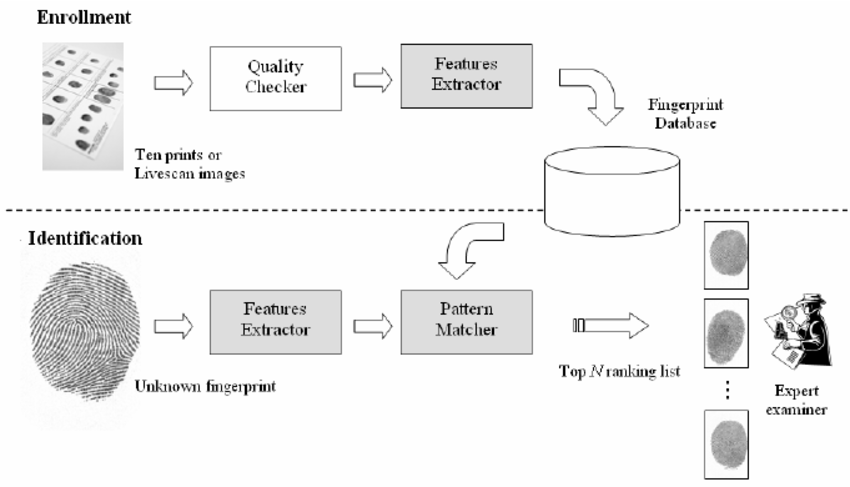
\includegraphics[width=.8\textwidth]{figures/AFIS.png}
	\caption{自动指纹识别系统框图 }\label{lssct}
\end{figure}

		\subsection{问题概述}
		    围绕相关附件和条件要求,试根据附件中的16幅指纹图像,不借助现有的指纹相关软件,依次提出以下问题:
				 
			\textbf{编码:} 给出一种用不超过200字节(下面称为“指纹密码”)来刻画描述指纹基本特征的表示方法,介绍其数学原理。
			
			\textbf{匹配:} 将你的方法编程实现,对附件中的每一幅指纹都给出其“指纹密码”的表示。基于你找到的这些指纹表示,你能否给出一种方法比较不同指纹间的异同及相似程度?
			
			\textbf{应用:} 你能否对附件中的16个指纹进行对比和归类?请给出你对比及分类的依据和结果。

	\section{模型假设}
		\begin{itemize}                                             
	\item [(1)] 假设附件中所有指纹图像都为清晰完整的图像,不存在由于图像压缩产生的信息损失。
\item [(2)] 假设附件中的指纹图像特征都具有代表性,具有正常人指纹拥有的所有特征。
		\item [(3)] 
		\item [(4)] 
		\end{itemize}

	\section{符号说明}
		\begin{table}[H]
		\centering
		\setlength{\tabcolsep}{12mm}
		\begin{tabular}{cc}
			\toprule[1.5pt]
			\multicolumn{1}{m{5cm}}{\centering 符号} & \multicolumn{1}{m{5cm}}{\centering 说明} \\
			\midrule[1pt]		
$b$  & 编码大小  \\ 
$b$  & 编码大小  \\ 
$b$  & 编码大小  \\ 
$b$  & 编码大小  \\ 
$b$  & 编码大小  \\ 
$b$  & 编码大小  \\ 
$X$  & 图像矩阵  \\ 
$\gamma$  & 编码器的图像编码  \\ 
$b$  & 编码大小  \\ 
$Z$  & 解码器还原的图像矩阵  \\ 
$epoch$  & 迭代次数  \\ 
$in/out$  & 出/入通道数  \\ 
  	$b$  & 编码大小  \\ 
$lr$  & 学习率  \\ 
$k_i$  & 卷积核i  \\ 
			\bottomrule[1.5pt]
		\end{tabular}
		\begin{tablenotes}
		\item 注:表中未说明的符号以首次出现处为准
		\end{tablenotes}
		\end{table}
	
	\section{数据预处理}
在正式搭建模型前,本文首先将图片进行预处理,以方便进行后续运算。经过归一化处理,图像增强处理和二值化处理后,即可得到相同规格的二值化图片,其具体流程如图~\ref{dfsg}~所示
\begin{figure}[H]
	\centering
	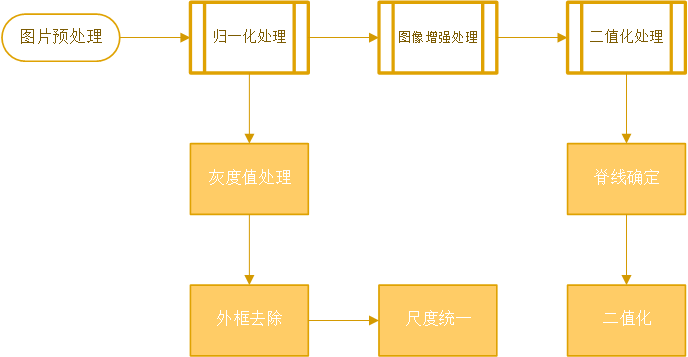
\includegraphics[width=.9\textwidth]{figures/chou4.png}
	\caption{图片数据预处理}\label{dfsg}
\end{figure}   
\subsection{归一化处理}
\subsubsection{灰度值处理}
鉴于各个指纹图像的纹理深浅不统一,首先对每张图片做灰度值归一化处理。对于图片$P_{i}$,其第$x$行第$y$列的像素点的灰度值可表示为$P_{i}(x,y)\in[0,255]$。即当$P_{i}(x,y)=255$时,$P_{i}(x,y)$为纯白色像素点;当$P_{i}(x,y)=0$时,$P_{i}(x,y)$为纯黑色像素点。对于任意图片$P_{i}$,有
\begin{gather*}
	P_{i,max}=\underset{1\leqslant x\leqslant n,1\leqslant y \leqslant  m}{max}P_{i}(x,y),\\
	P_{i,min}=\underset{1\leqslant x\leqslant n,1\leqslant y \leqslant  m}{min}P_{i}(x,y),
\end{gather*}
其中$n$和$m$分别表示图片的行数和列数。即	$P_{i,max}$与$P_{i,min}$分别表示图片中像素的最大灰度值和最小灰度值。对图片执行线性归一化操作如下
\begin{gather*}
	P_i(x,y)'=\frac{255}{P_{i,max}-P_{i,min}}(P_i(x,y)-P_{i,min}),
\end{gather*}
即将图片$P_i$像素点灰度值线性放缩于$[0,255]$间,得到灰度值归一化图片$P_i'$。

\subsubsection{外框去除与尺度统一}
对于图片$P_{i}$,我们将去除其空白外框以方便后续学习策略运算。设定边界阈值为$threshold_N$,当图片$P_{i}$最上方的某一行和最下方的某一行的非空白像素数大于$threshold_N$时,将其定义为新的上边界或下边界,及可得到行边界位置如下
\begin{gather*}
	fringe_{x1}=\underset{ (\sum_{i=1}^{m} (P'(x,i)<255))>threshold_N}{max(x)},\\
	fringe_{x2}=\underset{(\sum_{i=1}^{m} (P'(x,i)<255))>threshold_N}{min(x)},
\end{gather*}
其中$fringe_{x1}$与$fringe_{x2}$ 分别为新定义上边界与下边界,同理有列边界位置如下:
\begin{gather*}
	fringe_{y1}=\underset{(\sum_{i=1}^{n} (P'(i,y)<255))>threshold_N}{min(y)},\\
	fringe_{y2}=\underset{(\sum_{i=1}^{n} (P'(i,y)<255))>threshold_N}{max(y)},
\end{gather*}
其中$fringe_{y1}$与$fringe_{y2}$分别为新定义左边界与右边界。即去除外框后的图片可表示为	$P''=P'(	fringe_{x1}:	fringe_{x2},	fringe_{y1}:	fringe_{y2})$。即只保留新定义边界内的像素点并删除剩余像素点即可得到去除外框后的图片$P''_{i}$。定义标准行数为$N$,标准列数为$M$,将去除外框后的图片$P''_{i}$进行放缩处理可得归一化图片$P_{i}^s$如下:
\begin{gather*}
	P_{i}^s(x,y)=P''_{i}(floor(\frac{fringe_{x1}-fringe_{x2}}{N}x),floor(\frac{fringe_{y2}-fringe_{y1}}{M}y)),\\
	x\in[1,N],	y\in[1,M],
\end{gather*}
其中$floor$表示向下取整,即通过灰度值处理、外框去除与尺度统一后即可将原始指纹图片数据$P_{i}$转换为灰度值范围与图片尺度统一的归一化图片数据$P_{i}^s(x,y)$。
\subsection{图像增强处理}
利用Grunward-Letnikov微分算子\upcite{5},构造自适应函数,采集梯度信息和计算信息熵,从而确定微分阶数。	
为了确定自适应分数阶微分阶数$v$,需要确定每个像素的梯度$G$和信息熵$E$。
梯度$G$反映指纹像素特征在感兴趣区域(ROI, Region of Interest)上的突变情况,取近似梯度模值为
\begin{gather}
	\displaystyle G[P(x,y)]=\max\begin{Bmatrix}
		|\frac{\partial P }{\partial x}|,|\frac{\partial P}{\partial y}|
	\end{Bmatrix}.
\end{gather}

另一个描述图像边缘纹理变化的指标是信息熵$E$,即所有可能发生事件的信息量期望之和,其数学描述为
\begin{gather}
	E=-\sum_{i=1}^{n}p(x_i)\cdot log_2(p(x_i)),	
\end{gather}
其中,$p(x_i)$是事件$x_i$发生的概率,$n$是可能发生事件的个数。对信息熵进行归一化处理,可以获得取值范围为$[0,1]$的信息熵
\begin{gather}
	\displaystyle E'=\frac{E-E_{min}}{E_{max}-E_{min}}.
\end{gather}

综合梯度模值和信息熵,构造关系函数$v=w_1\cdot G+w_2\cdot E'+w_3$,即微分阶数$v$由梯度和信息熵共同决定,梯度模值和信息熵越大,反映该指纹像素需要增强的程度越大,更可能为纹理区域或边缘,分数阶微分阶数取值也越大。此问题中,可算得$v=3$。将阶数代入利用Grunward-Letnikov分数阶微分近似表达式,即

\begin{gather}
	\displaystyle\frac{\partial^v P(x,y)}{\partial x_{i}^{v}}\doteq\displaystyle\sum_{k=0}^{t-\alpha}(-1)^{k}\begin{pmatrix}
		v \\ k
	\end{pmatrix}P(x_i-k), 
\end{gather}
其中$P(x,y)$是图像坐标为$(x,y)$的像素灰度值,$t$和$\alpha$分别是微分上限和下限,$x_i(i=0,1,...,7)$是不同的偏微分方向,此处取以$x$轴正向为起始方向,顺时针旋转一周均匀分部的$8$个方向。为方便计算,对$8$个方向的分数阶偏微分近似分别保留前三项进行三层$5 \times 5$掩膜构造,并进行归一化赋权。

对每个方向$x_i$,以掩膜中心点为作用点,$5\times 5$掩膜$w(x,y)$中三层权重分别为分数阶微分近似的前三项系数,则掩膜中总权重为分数阶微分近似的前三项系数与每层掩膜元素个数的乘积之和,即$4v_2-12v+8$。对权重归一化,可得中心点、第一层、第二层掩膜元素权重分别为$\displaystyle w_0=\frac{8}{4v_2-12v+8}, w_1=\frac{-v}{4v_2-12v+8}, w_2=\frac{v}{16(v-2)}$。
在规模为$M\times N$的图像上,对距离中心点小于$\displaystyle M-\frac{n-1}{2}$和$\displaystyle N-\frac{n-1}{2}$的像素进行$n\times n$掩膜操作,其他像素进行灰度保留。输出图像可以表示为:
\begin{gather}
	\displaystyle g(x,y)=\sum_{s=-a}^{a}\sum_{t=-b}^{b}P(x+s,y+t)\cdot \boldmath{w}(x,y),
\end{gather}
其中,$w(x,y)$是构造的$5\times 5$掩膜,$a=b=\displaystyle \frac{n-1}{2}$。


\subsection{二值化处理}	  	
\subsubsection{场方向估计}
一般指纹图像都有较为清晰的场方向,对于图像上的每一个像素$P(x,y)$,为了确定其在该像素处脊线的方向,以该像素为中心的$9\times9$像素矩阵$u_{P(x,y)}$内,分别计算$8$个
方向上的灰度平均值\upcite{6},即对于
\begin{gather*}
	u_{P(x,y)}=\begin{bmatrix}
		P(x-4,y-4) & \cdots  & P(x,y-4) & \cdots  & P(x+4,y-4) \\ 
		\vdots & \udots & \vdots  &  \ddots  & \vdots\\ 
		P(x-4,y) & \cdots & P(x,y) &\cdots& P(x+4,y)  \\ 
		\vdots & \ddots  & \vdots  &  \udots & \vdots\\ 
		P(x+4,y+4) & \cdots & P(x,y+4) &\cdots& P(x+4,y+4)  
	\end{bmatrix}.
\end{gather*}

若$u_{P(x,y)}$中存在若干像素点超出原图像边界时,记超出边界的像素点为$P_o$并使得$\left \{ P_o \right \}=255$。并依照图~\ref{adf}~中的方向,分别计算$8$个方向上的灰度平均值得到$Gmean[i]$,然后将这 $8$ 个平均值按两两垂直的方向分成 $4$ 组,$0 $和 $4$ 一组、$1$ 和 $5$ 一组、$2$ 和 $6$ 一组、$3$ 和 $7$ 一组,计算
每组中两个平均值的差值。
\begin{gather*}
	Gdiff[j]=\left | Gmean[j]-Gmean[j+4] \right |,j=1,2,3,4,
\end{gather*}
差值绝对值相差最大的方向即为脊线方向与其法向,即
\begin{gather*}
	iDir=\left\{\begin{matrix}arg(\underset{i}{max}(Gdiff[j])),\left | P(x,y)-\underset{i}{max}(Gdiff[j]) \right|<\left | P(x,y)-\underset{i}{max}(Gdiff[j+4]) \right|
		\\ arg(\underset{i}{max}(Gdiff[j]))+4,otherwise
	\end{matrix}\right.
\end{gather*}
\begin{figure}[H]
	\centering
	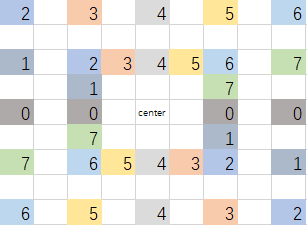
\includegraphics[width=.5\textwidth]{figures/chou.png}
	\caption{脊线估计方向}\label{adf}
\end{figure}   
\subsubsection{二值化}
得到图像每个像素处的方向场后,再依据方向场来对图像进行二值化。若像素$P(x,y)$处的脊线方向为$iDir$,先用估计方向场的方法计算该像素处在方向$iDir$和其法线$iVar=iDir+4$的灰度平均值$ Gmean[iDir]$和$ Gmean[iVar]$,基于此将该像素二值化为
\begin{gather*}
	P(x,y)=\left\{\begin{matrix}255, Gmean[iDir]\geqslant Gmean[iVar]
		\\ 0,otherwise
	\end{matrix}\right. ,
\end{gather*}
其中255为二值图像中图像背景和谷线的灰度值,0 为二值图像中图像脊线的灰度值。

	经过上述处理指纹图像,得到最终结果如图所示
	       	\begin{figure}[H]	
		\centering
		\subfigure[指纹原始图像]{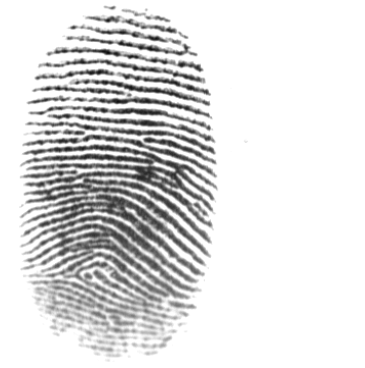
\includegraphics[height=5cm,width=5cm]{figures/rrr.png}}
		\subfigure[指纹预处理后]{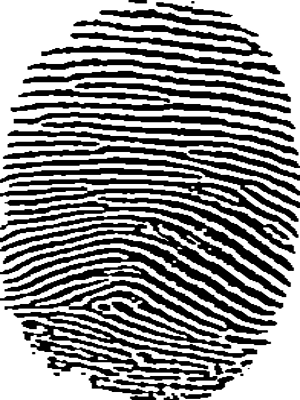
\includegraphics[height=5cm,width=3cm]{figures/result01.png}}
		\caption{图像预处理的效果图}
		\label{zhiwesn}
	\end{figure}
	
	
	\section{问题一模型的建立与求解}
	
		\subsection{问题描述与分析}
			问题一要求给出一种用不超过200字节来刻画描述指纹基本特征的表示方法。传统的图像压缩方法有霍夫曼压缩、Golomb编码、LZW编码、小波编码等\upcite{7,8,9},这些都能对指纹进行刻画。但是相对于200字节的限制而言,他们在压缩编码方向显得不尽人意。
			
			相较于传统的图片编码而言,通过网络编码能更有效的提高图像在细节上的依赖。在网络训练的过程中,网络只用到该向量之中少量元素,其中的大部分元素对于网络来说是没有用的。自编码器通过无监督学习来提取有用的信息,对于指纹图片来说是颜色为黑色的像素点,将图片中的很大一部分白色像素舍弃,只提取对网络有用的信息,到达降低数据维度的目的,从而实现小样本编码。
		
%			其思维流程图如图~\ref{lct}~所示:
%			\begin{figure}[H]
%				\centering
%				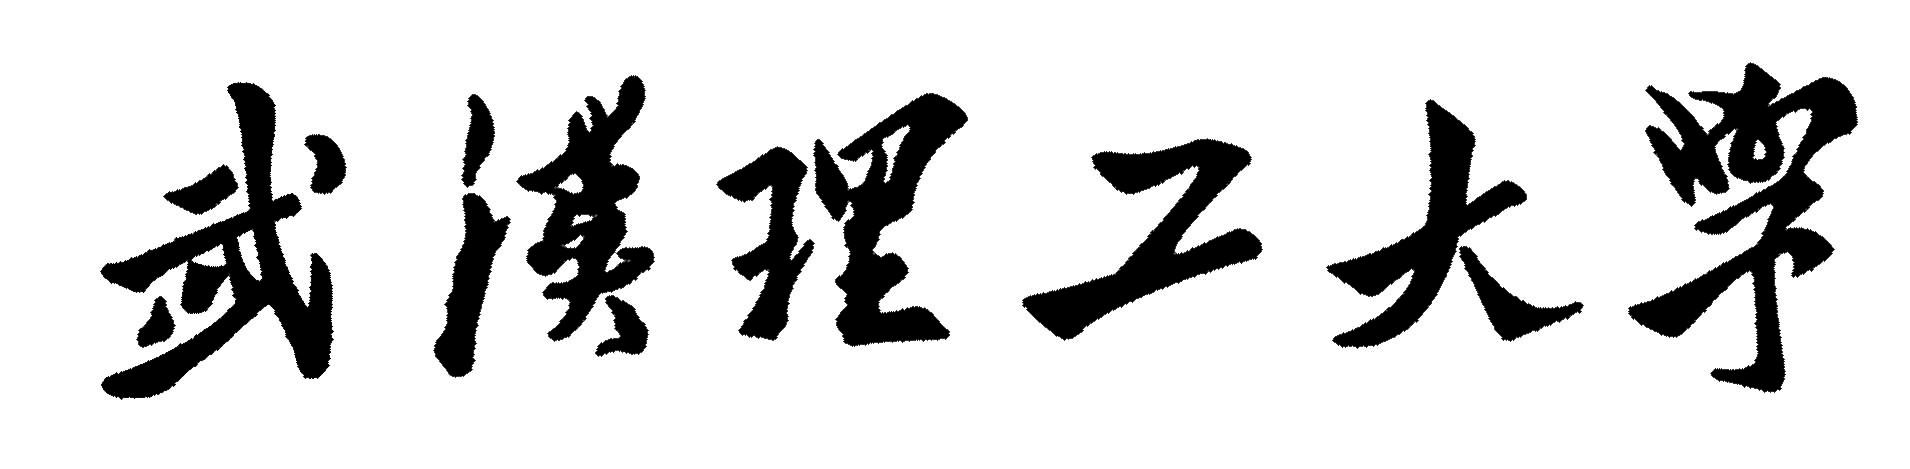
\includegraphics[width=\textwidth]{figures/whut.jpg}
%				\caption{问题一思维流程图}\label{lct}
%			\end{figure}
%			
		\subsection{搭建卷积自编码器模型}
		   自编码器(AutoEncoder)是一种能够通过无监督学习,学到输入数据高效表示的人工神经网络。输入数据的这一高效表示称为编码(codings),其维度一般远小于输入数据,使得自编码器可用于降维\upcite{10}。更重要的是,自编码器可作为强大的特征检测器(feature detectors),应用于深度神经网络的预训练。我们以VGG模型\upcite{4}结构为基础,构造一个 新的卷积神经网络模型,并通过交叉验证的思想训练小样本数据,调整
		   模型参数,得到小样本条件下最优的卷积神经网络模型。
		
			\subsubsection{卷积神经网络}
			
			\paragraph{Convolution Kernel} 在图像处理的过程中,我们经常会用到矩阵卷积来计算图像(image)的特征(feature),矩阵卷积有两种:全卷积(full convolution)和有效值卷积(valid convolution)\upcite{11},其全卷积核函数的定义式为:
			     \begin{gather}
z(u, v)=\sum_{i=-\infty}^{\infty} \sum_{j=-\infty}^{\infty} x_{i, j} \cdot k_{u-i, v-j},
			     \end{gather}
			有效值卷积的定义式为:
			\begin{gather}
\begin{array}{c}
z(u, v)=\displaystyle\sum_{i=-\infty}^{\infty} \sum_{j=-\infty}^{\infty} x_{i+u, j+v} \cdot k_{r o t i, j} \cdot \chi(i, j) \\
\chi(i, j)=\left\{  
\begin{array}{c}
1,0 \leqslant i, j \leqslant n \\
0, \text {others}
\end{array}
\right.  
\end{array},
			\end{gather}
			其中$X$是灰度图像转换为$m\times m$阶矩阵,$K$是$n\times n$阶卷积核,一般取$3\times 3$,$K_{rot}$是由$K$转置得到。
			
		那么,从 Input Image 到 Output Image 的变化如下图所示:
		\begin{figure}[H]
			\centering
			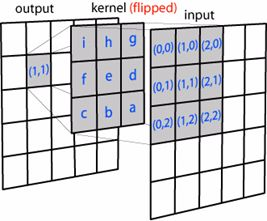
\includegraphics[width=.5\textwidth]{figures/cnn.jpg}
			\caption{卷积核函数示意图}
		\end{figure}
		可以看出,其实二维卷积一样也是加权叠加/积分。需要注意的是,其中 Convolution Kernel 进行了水平和竖直方向的翻转。
		
			\paragraph{Pooling} 对于灰度图像的采样而言,Pooling 对于输入的 Feature Map,选择某种方式对其进行压缩。如下图,表示的就是对$2\times 2$邻域内的值,选择最大值输出到下一层,这叫做 Max-Pooling。
				\begin{figure}[H]
			\centering
			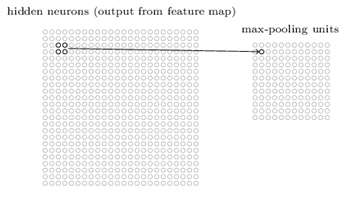
\includegraphics[width=.5\textwidth]{figures/pool.png}
			\caption{池化层Max-Pooling示意图}
		\end{figure}
	
	对卷积层进行池化从而通过对 Feature Map 降维,有效减少后续层需要的参数,当其中像素在邻域发生微小位移时,Pooling Layer 的输出是不变的。这就增强了网络的鲁棒性,有一定抗扰动的作用。
	
	\paragraph{Activation} 激活层的正向传播主要依靠众多神经元的计算来完成的,工作过程中可以用下式来表示:
	\begin{gather*}
	{u_{k}=\sum_{i=1} w_{k i} x_{i}}, \\ {y_{k}=f\left(u_{k}-b_{k}\right)},
	\end{gather*}
	其中:$x_{i}$表示第 i 个输入; $w_{ki}$表示与第 i 输入量相连的权值;$u_{k}$表示所有输入的加权和;$b_{k}$为神经 元阈值;$ f$ 为激活函数;$y_{k}$ 为神经网络的输出。
	
	激活函数的种类有很多,如 $sigmoid$, $tanh$ 及$ Relu$,本文应用的是 $Relu$作为激活函数搭建两层隐含层,如式~\ref{shiw}~所示:
	\begin{gather}\label{shiw}
	\begin{array}{c}{f_{\text {Relu}}=\max (0, z)}\\
	\displaystyle \frac{d}{d z} f_{R e L U}=\left\{\begin{array}{ll}{1,} & {z>0} \\ {0,} & {z \leqslant 0}\end{array}\right.
	\end{array}.
	\end{gather}
	
	网络的输出层使用$ softmax $函数作分类器, 式~\ref{shiq}~为第 i 个神经的输出:
	\begin{gather*}\label{shiq}
	f_{\text {softmax}}=\mathrm{e}^{i} / \sum_{j} \mathrm{e}^{j}.
	\end{gather*}
	
			\subsubsection{卷积自动编码器}
			普通的自编码器中,编码器和解码器中层与层之间的连
			接方式为全连接,该编码器具有一个输入层,n个隐藏层和一个输出层,
			
			给定图片样本$X=\left\{ x_1,x_2,\cdots,x_nx \right\}, X\in \mathbb{R}^{n\times c\times w \times h}$,其中c为通道数。自编码器首先将$x_i$编码成$\gamma(x_i)$再解码成$z(y_i)$,其公式L表述如下:
				\begin{gather}
			\begin{array}{l}
			\gamma (x)=Encoder\left(W_{1} x+b\right) \\
			z(x)=Decoder\left(W_{2} y(x)+c\right)
			\end{array}.
			\end{gather}
			
			通过最小化重建误差$L(X,Z)$,我们可以获得模型参数,这里用θ表示为:
			\begin{gather}
			\theta=\underset{\theta}{\arg \min } L(X, Z)=\underset{\theta}{\arg \min } \frac{1}{2} \sum_{i=1}^{N}\left\|x^{(i)}-z\left(x^{(i)}\right)\right\|^{2}.
			\end{gather}

			本文卷积自编码器(ConvAutoEncoder, CAE)中的编码器部分的网络结构与卷积神
			经网络中卷积池化部分的结构相同。首先通过编码器部分构
			造出对应的解码器部分,在训练结束后,保留编码器部分的结
			构和权重,在编码器后加上与卷积神经网络结构中相同的全
			连接层来进行图像的编码与分类识别\upcite{12,13}。其卷积自编码器$L(X,Z)$的具体结构如图
			\ref{labssel}所示:
					\begin{figure}[H]
				\centering
				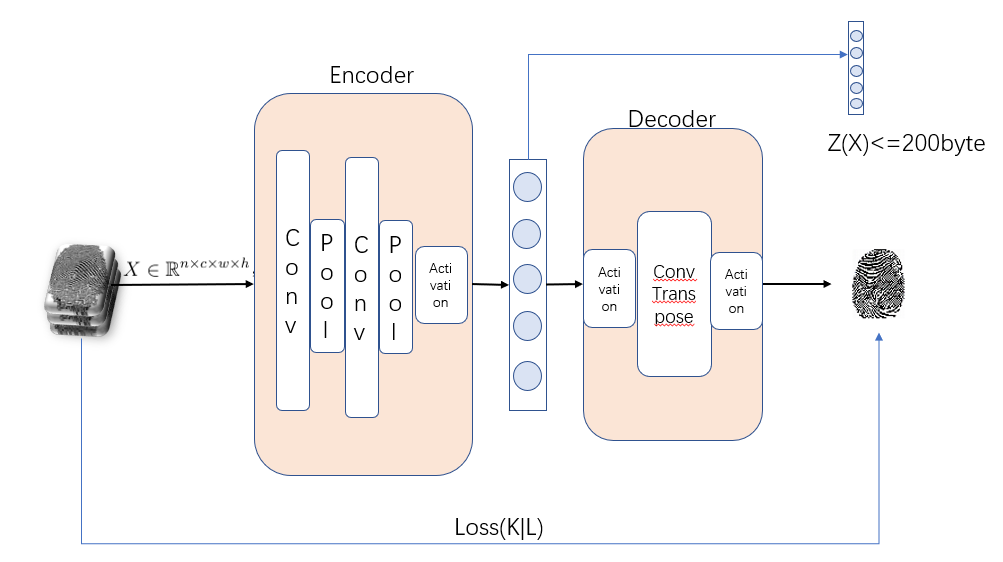
\includegraphics[width=\textwidth]{figures/model.png}
				\caption{卷积自编码器CAE模型}\label{labssel}
			\end{figure}
		其中,Conv表示全卷积,ConvTranspose表示有效值卷积,Activation表述rule激活层,Pooling表示池化层,对应的编码输入为$Z(X)<200byte$。
		
	
					将稀疏约束添加到目标函数后,自动编码器将成为稀疏的自动编码器,它考虑二值图像隐藏层的稀疏表示。 为了实现稀疏表示,本文将使用稀疏约束将重构误差最小化,加上损失函数KL散度:
								\begin{gather}
					 \mathrm{CAE}=L(X, Z)+\gamma \sum_{j=1}^{H_{D}} \mathrm{KL}\left(\rho \| \hat{\rho}_{j}\right),\\
					 \mathrm{KL}\left(\rho \| \hat{\rho}_{j}\right)=\rho \log \frac{\rho}{\hat{\rho}_{j}}+(1-\rho) \log \frac{1-\rho}{1-\hat{\rho}_{j}},
								\end{gather}
					其中γ是稀疏项的权重,$H_D$是隐藏单元的数量,ρ是稀疏性参数,通常是一个接近零的小值。$\hat{\rho}_{j}=(1 / N) \sum_{i=1}^{N} y_{j}\left(x^{(i)}\right)$是在训练集中隐藏单元j的平均激活。

在迭代修正的过程中,实验采用$Keras$自带优化器Adam函数进行迭代修正,如式~\ref{adam}~所示,其中$\beta_{1}$一般取0.9,$\beta_{2}$一般取0.999。

\begin{gather*}\label{adam}
\left\{\begin{array}{l}{m_{t}=\beta_{1} m_{t-1}+\left(1-\beta_{1}\right) \nabla_{w} f\left(w_{t}\right)} \\ {v_{t}=\beta_{2} v_{t-1}+\left(1-\beta_{2}\right) \nabla_{w} f\left(w_{t}\right)^{2}} \\ {\widehat{m}_{t}=\frac{m_{t}}{1-\beta_{1}^{t}}, \hat{v}_{t}=\frac{v_{t}}{1-\beta_{2}^{t}}} \\ {w_{t}=w_{t-1}-\eta \frac{\widehat{m}_{t}}{\sqrt{\hat{v}_{t}+\varepsilon}}}\end{array}\right.
\end{gather*}

        \subsection{实验结果及分析}
        实验训练输入样本为 400×300的指纹图片, 具体参数设置如表所示:
       \begin{table}[H]
        	\setstretch{1.4}  %设置表的行间距
        	\centering		
        	\caption{参数设置表
        	}
        	\begin{tabular}{cc|cc}
        		\toprule[1.5pt]
        		\multicolumn{1}{m{5cm}}{\centering 参数名称}
        		& \multicolumn{1}{m{2cm}}{\centering 值}
        		& \multicolumn{1}{m{5cm}}{\centering 参数名称}
        		& \multicolumn{1}{m{2cm}}{\centering 值}
        		\\
        		\midrule[1pt]
        		迭代次数 epoch&   2000& 吞吐量 batch & 64\\ 
        	出/入通道数 in/out& 	3/3& 编码大小 size& 200\\
        	        学习率 lr& 0.01& 偏置 $\beta_1,\beta_2$& 0.9, 0.999\\
      卷积核 $k_1,k_2,k_3$& 3,3,4& 池化层 padding& 1\\
        		\bottomrule[1.5pt]	
        	\end{tabular}
        \end{table}
    
        通过上述参数设置,计算16张指纹图片KL散度的最小值,并保存其编码程序。其迭代过程中 损失函数如下图所示:
        	\begin{figure}[H]
        	\centering
        	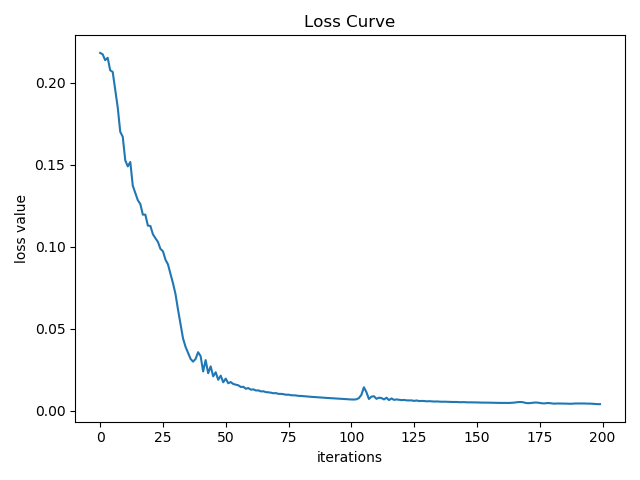
\includegraphics[width=.6\textwidth]{figures/loss.png}
        	\caption{CAE迭代过程中损失函数函数}\label{loss}
        \end{figure}
    可以看出,我们的模型在解码还原过程中,能明显逼近于真实的指纹图片,信息损失仅占0.04\%,对于传统的编码方法有明显的压缩能力。
    
    本文将指纹编码过程进行还原,得到解码图像入下图所示,图中的指纹图像上方数字表示迭代次数,显然随迭代次数增加,还原的指纹图像的清晰度与完整度逐渐增加;当迭代次数超过120时,图像清晰度变化几乎无法用肉眼分辨。显然经由CAE模型编码后的指纹图像可被高精度还原。
       	\begin{figure}[H]	
        	\centering
        	\subfigure[指纹1过程过程]{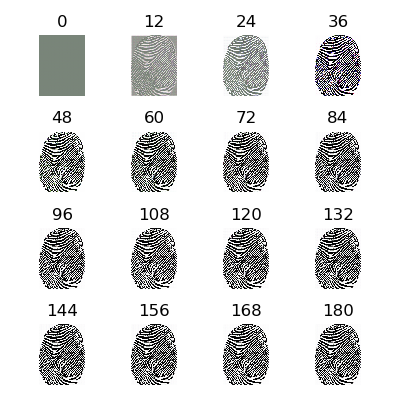
\includegraphics[height=8cm,width=7.5cm]{figures/zhiwen.png}}
        	\subfigure[指纹2解码过程]{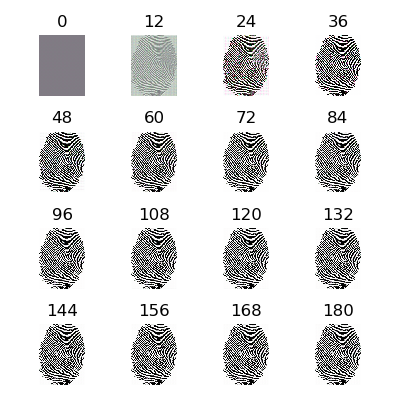
\includegraphics[height=8cm,width=7.5cm]{figures/zhiwen2.png}}
        	\caption{编码后经解码器后还原的效果图}
        	\label{zhiwen}
        \end{figure}
    
    

	\section{问题二模型的建立与求解}
		\subsection{问题分析与相似度计算}

问题二要求从第一问求得的指纹编码的角度分析各个指纹间的异同及相似程度。在使用卷积自动编码器将原始指纹图像转化成了特征编码后,图像的特征编码是以能反映指纹特征的行向量存储。对各行向量的每一维度进行归一化处理,分别计算归一化后的行向量间的谷本系数(Tanimoto Coefficient)、皮尔森相关系数(Pearson Correlation Coefficient)和马哈拉诺比斯距离(Mahalanobis Distance),最后构造关系函数确定行向量的相似程度。
			
			
			\begin{itemize}
				\item \textbf{谷本系数(Tanimoto Coefficient)}
				
				谷本系数主要用于计算符号度量或布尔值度量的个体间的相似度,因为个体的特征属性都是由符号度量或者布尔值标识,因此无法衡量差异具体值的大小,只能获得“是否相同”这个结果,所以谷本系数只关心个体间共同具有的特征是否一致这个问题。其数学描述为
				\begin{gather}
				T(A,B)=\frac{A\ast B}{\begin{Vmatrix}
						A
					\end{Vmatrix}^2+\begin{Vmatrix}
						B
					\end{Vmatrix}^2-A\ast B}
				\end{gather}
				其中$\begin{Vmatrix}
				A
				\end{Vmatrix}^2$和$\begin{Vmatrix}
				A
				\end{Vmatrix}^2$分别是行向量$A$和$B$的模。
				\item \textbf{皮尔逊相关系数(Pearson Correlation Coefficient)}\\
				皮尔逊相关系数反应了两个变量之间的线性相关程度,它的取值在[-1, 1]之间。
				\begin{gather}
					P(A,B)=\frac{cov(A,B)}{\sigma_A\cdot \sigma_B}
				\end{gather}
				其中$cov(A,B)$是行向量$A$和$B$的协方差,$\sigma_A$和$\sigma_B$分别是$A$和$B$的元素标准差。
				\item \textbf{马哈拉诺比斯距离(Mahalanobis Distance)}\\
				马氏距离是一种距离的度量,可以看作是欧氏距离的一种修正,修正了欧式距离中各个维度尺度不一致且相关的问题。
				\begin{gather}
				M(A,B)=\sqrt{(A-B)^T\Sigma^{-1}(A-B)}
				\end{gather}
			\end{itemize}
			其中,$\Sigma$是随机变量的协方差矩阵。
			
			构造关系函数如下所示,用$S(A,B)$表示CAE输出行向量$A$和$B$的相似度:
			\begin{gather}
			S(A,B)=\omega_1 T(A,B)+\omega_2 P(A,B)+\omega_3 M(A,B)
			\end{gather}
			式中取$\omega_1=0.95$,$\omega_2=0.02$,$\omega_3=0.03$。



        \subsection{实验结果及分析}
        


    \section{问题三模型的建立与求解}

  	\subsection{问题描述与分析}
  	问题三在问题二将指纹相似度量化的基础上,进一步要求将样本指纹进行类比归类,其本质是一个样本分类问题。根据第二问的相似度量化结果,可得到任意两个指纹样本间的相似程度,即可在其基础上搭建中心聚类模型以将样本指纹进行类比归类。
  	
    本文设计的加权相似度$S$具有非欧几里得特征(引用),不可使用样本均值作为聚类中心,即不可使用经典中心聚类算法$k-means$算法经行样本聚类。针对该问题,我们引入$k-medoids$算法以确定样本中心点,并以模型二设计的加权相似度的平均值作为代价函数,对附件中的$16$个指纹样本进行聚类。
  	
  	\begin{figure}[H]
  		\centering
  		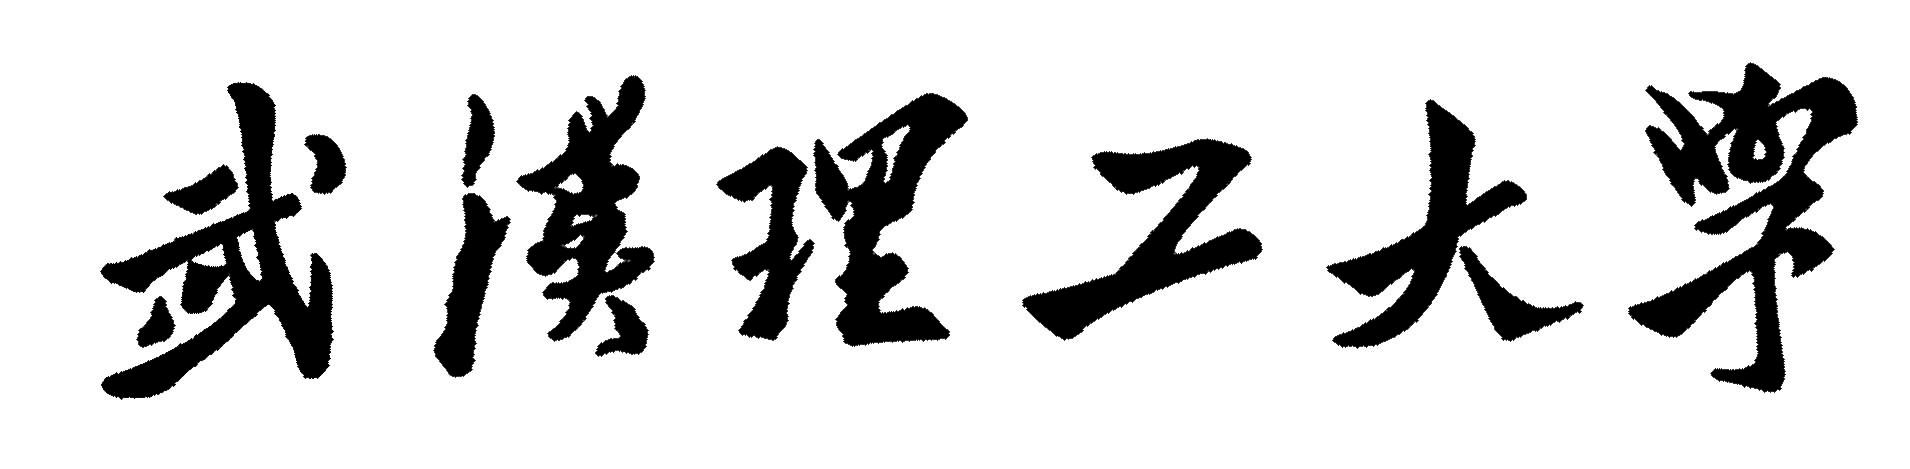
\includegraphics[width=\textwidth]{figures/whut.jpg}
  		\caption{问题二思维流程图}\label{lsssscst}
  	\end{figure}
  	\subsection{k-medoids模型的建立与求解}
  	本文采用$k-medoids$模式选取聚类中心点\upcite{14,15},从$16$个样本点$\left \{ \gamma_i  \right \}$中选取$k$个样本点作为聚类中心$\left \{ c_i \right \}$,即可求出代价函数为
  	\begin{gather}
  J(c_1,c_2,\cdots,c_k)=\frac{1}{16}\sum _{i=1}^{16}\underset{1\leqslant j\leqslant k}{Max}S(\gamma _i,c_j),
  	\end{gather}
  	其中$\underset{1\leqslant j\leqslant k}{Max}S(\gamma _i,c_j)$表示与样本点$ \gamma_i $与$k$个聚类中心$\left \{ c_i \right \}$间的最高的相似度值,即将$\gamma _i$归入与其相似度最高的聚类中心。即将聚类中心$\left \{ c_i \right \}$作为决策变量,搜索最佳聚类中心组合,使得代价函数$J(c_1,c_2,\cdots,c_k)$达到最大值,即
      	\begin{gather}
      max \frac{1}{16}\sum _{i=1}^{16}\underset{1\leqslant j\leqslant k}{Max}S(\gamma _i,c_j),\\
      s.t.\left \{  c_j  | j\in [1,k] \right \}  \subseteq  \left \{ \gamma _i | i\in [1,16]\right \} 
      \end{gather}
  	鉴于该问题样本规模较小,本文采用遍历方式,输入所有聚类中心并选取代价函数值最高的聚类中心组合
  	\subsection{实验结果及分析}

  
  	\section{灵敏度分析}
  本文对卷积自编码器中编码层输入的$\gamma$大小$b$做调整,得到
  				\begin{figure}[H]
  		\centering
  		\subfigure[$b \leq 10 \boldsymbol{byte} $]{
\includegraphics[height=3.5cm,width=3cm]{figures/guo/f1.png}}
  		\subfigure[$b \leq 50 \boldsymbol{byte} $]{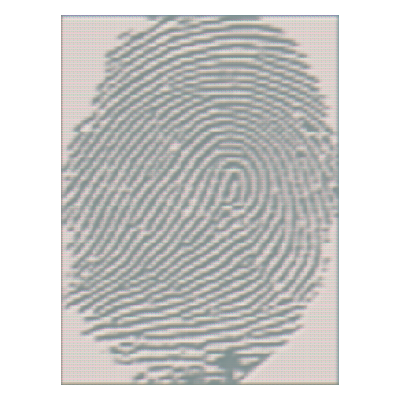
\includegraphics[height=3.5cm,width=3cm]{figures/guo/f2.png}}
  		\subfigure[$b \leq 100 \boldsymbol{byte} $]{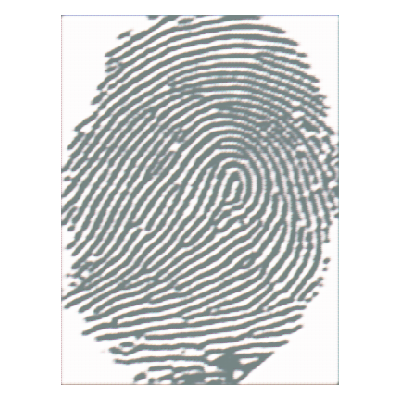
\includegraphics[height=3.5cm,width=3cm]{figures/guo/f3.png}}
  		\subfigure[$b \leq 120 \boldsymbol{byte} $]{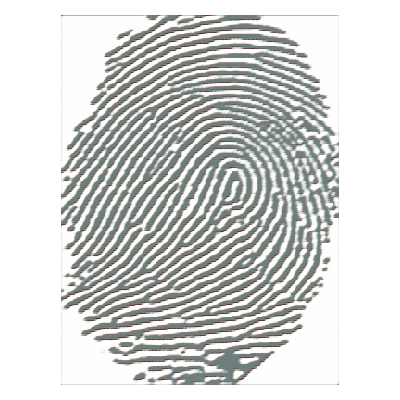
\includegraphics[height=3.5cm,width=3cm]{figures/guo/f4.png}}
  	\end{figure}	
  	\begin{figure}[H]	
  		\centering
  		\subfigure[$b \leq 150 \boldsymbol{byte} $]{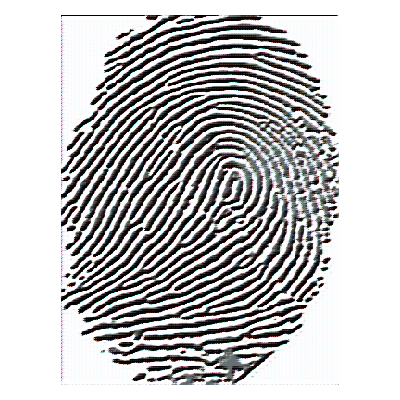
\includegraphics[height=3.5cm,width=3cm]{figures/guo/f5.png}}
		\subfigure[$b \leq 200 \boldsymbol{byte} $]{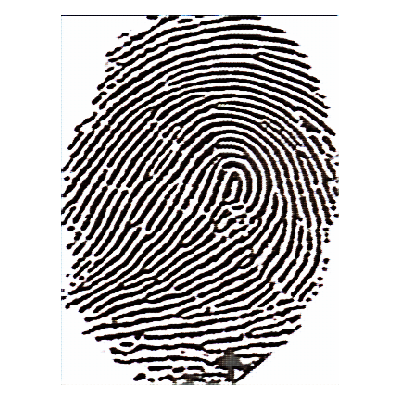
\includegraphics[height=3.5cm,width=3cm]{figures/guo/f6.png}}
		\subfigure[$b \leq 300 \boldsymbol{byte} $]{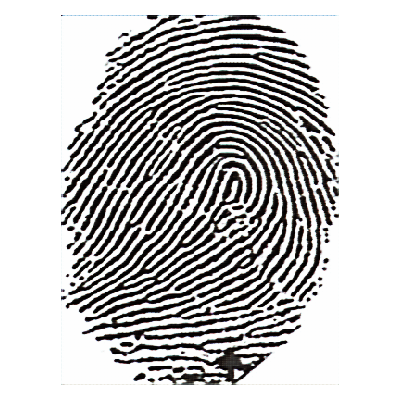
\includegraphics[height=3.5cm,width=3cm]{figures/guo/f7.png}}
		\subfigure[$b \leq 500 \boldsymbol{byte} $]{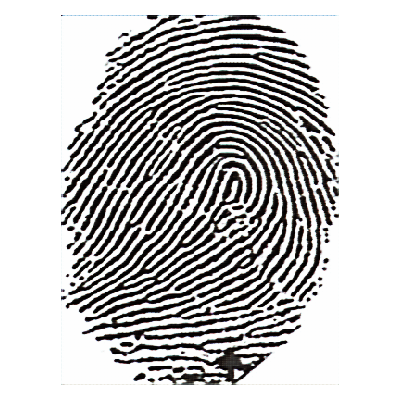
\includegraphics[height=3.5cm,width=3cm]{figures/guo/f8.png}}
  		\caption{编码不同字节限制后对应的解码指纹效果}
  		\label{fisg}
  	\end{figure}
  	根据上述解码后效果图可以看出:编码50字节后能还原出指纹大致轮廓,但是具体图像仍然不清晰;编码100字节能还原出微细节轮廓,但上方密集部分仍然呈现模糊状况;编码150字节后能较为清晰的还原,但还是存在少量噪声;而到200字节以上非常清晰,能通过降维后的编码数据完美的还原出原始指纹图像。
 	
  	\section{模型的评价}
		\subsection{模型的优点}
			\begin{itemize}                                             
			\item [(1)] 与传统编码而言,卷积自编码器通过无监督学习来提取指纹细节依赖充分压缩指纹图像,对于指纹图片来说是颜色为黑色的像素点,将图片中的很大一部分白色像素舍弃,只提取对网络有用的信息,到达降低数据维度的目的,并且在编码后能通过解码器还原出原始图像数据。
			\item [(2)] 	
			\end{itemize}
		\subsection{模型的缺点}

  		\subsection{模型改进}

  
  
 
	\newpage	%换页符
	%%参考文献
	%\begin{thebibliography}{9}%宽度9
	% \setlength{\itemsep}{-2mm}
	\nocite{*}		%排版未引用的参考文献
	\begin{thebibliography}{9}%宽度9
		\bibitem{1}Davies S G. Touching Big Brother: How biometric technology will fuse flesh and machine[J]. Information Technology \& People, 2014, 7(4): 38-47.
	\bibitem{2}Moses K R, Higgins P, McCabe M, et al. Automated fingerprint identification system (AFIS)[J]. Scientific Working Group on Friction Ridge Analysis Study and Technology and National institute of Justice (eds.) SWGFAST-The fingerprint sourcebook, 2011: 1-33.
	\bibitem{3}Dror I E, Wertheim K, Fraser‐Mackenzie P, et al. The impact of human–technology cooperation and distributed cognition in forensic science: biasing effects of AFIS contextual information on human experts[J]. Journal of forensic sciences, 2012, 57(2): 343-352.
	\bibitem{4}Simonyan K, Zisserman A. Very deep convolutional networks for large-scale image recognition[J]. arXiv preprint arXiv:1409.1556, 2014.
	\bibitem{5}Scherer R, Kalla S L, Tang Y, et al. The Grünwald–Letnikov method for fractional differential equations[J]. Computers \& Mathematics with Applications, 2011, 62(3): 902-917.
	\bibitem{6}邓正宏, 丁有军. 基于动态方向场的指纹图像增强算法[J]. 微电子学与计算机, 2005, 22(2): 70-72.
	\bibitem{7}蓝波, 林小竹, 籍俊伟. 一种改进的 LZW 算法在图像编码中的应用[J]. 计算机工程与科学, 2006, 28(6): 55-57.
	\bibitem{8}张旭东. 图像编码基础和小波压缩技术: 原理, 算法和标准[M]. 清华大学出版社有限公司, 2004.
	\bibitem{9}赵利平, 林涛, 周开伦. 屏幕图像压缩中串复制位移参数的高效编码算法[J]. 计算机学报, 2017, 40(5): 1218-1228.
	\bibitem{10}黄健航, 雷迎科. 基于边际 Fisher 深度自编码器的电台指纹特征提取[J]. 模式识别与人工智能, 2017 (2017 年 11): 1030-1038.
	\bibitem{11}Gao L, Chen P Y, Yu S. Demonstration of convolution kernel operation on resistive cross-point array[J]. IEEE Electron Device Letters, 2016, 37(7): 870-873.
	\bibitem{12}Guo X, Liu X, Zhu E, et al. Deep clustering with convolutional autoencoders[C]//International conference on neural information processing. Springer, Cham, 2017: 373-382.
	\bibitem{13} 王万良, 杨小涵, 赵燕伟, 等. 采用卷积自编码器网络的图像增强算法[J]. 浙江大学学报 (工学版), 2019, 53(9): 1728-1740.
	\bibitem{14}Arora P, Varshney S. Analysis of k-means and k-medoids algorithm for big data[J]. Procedia Computer Science, 2016, 78: 507-512.
	\bibitem{15}Yu D, Liu G, Guo M, et al. An improved K-medoids algorithm based on step increasing and optimizing medoids[J]. Expert Systems with Applications, 2018, 92: 464-473.
	\end{thebibliography}

	\newpage
	%附录
	\appendix %%附录
	\section{数据预处理}
\subsection*{去噪--matlab源代码}
\begin{lstlisting}[language=matlab]
imdata=imread('01.tif');
imshow(imdata);
flag=0;
Min=min(min(imdata));
Max=max(max(imdata));
h=medfilt2(imdata);%去噪
for i=1:size(imdata,1)
for j=1:size(imdata,2)
if (h(i,j)>200)
h(i,j)=255;
end
end
end
h1=histeq(h);%增强
subplot(221);imshow(imdata);
subplot(222);imshow(h);
subplot(223);imshow(h1);

for i=1:size(imdata,1)
for j=1:size(imdata,2)
if (imdata(i,j)<255)
fringe_x1=i;
flag=1;
break;
end
end
if(flag==1)
flag=0;
break;
end
end
for i=size(imdata,1):-1:1
for j=1:size(imdata,2)
if (imdata(i,j)<255)
fringe_x2=i;
flag=1;
break;
end
end
if(flag==1)
flag=0;
break;
end
end
for i=1:size(imdata,2)
for j=1:size(imdata,1)
if (imdata(j,i)<255)
fringe_y1=i;
flag=1;
break;
end
end
if(flag==1)
flag=0;
break;
end
end
for i=size(imdata,2):-1:1
for j=1:size(imdata,1)
if (imdata(j,i)<255)
fringe_y2=i;
flag=1;
break;
end
end
if(flag==1)
flag=0;
break;
end
end
% image=imdata(  fringe_x1:   fringe_x2 ,fringe_y1:  fringe_y2);
% subplot(224); imshow(image);
\end{lstlisting}
		\subsection*{处理图像--matlab源代码}
	\begin{lstlisting}[language=matlab]
	f=imread('16.tif');%读取图像到内存
	%f=imresize(f,[363,312]);%该函数用于对图像做缩放处理。
	%figure;imshow(f);
	%用rgb2gray 将彩色图像转换为灰度图像。matlab读入图像的数据是uint8,而matlab中数值一般采用double型(64位)存储和运算。
	%所以要先将图像转为double格式的才能运算
	gray=double((f));
	%转成uint8 imshow()显示图像时对double型是认为在0~1范围内即大于1时都是显示为白色,而imshow显示uint8型时是0~255范围。
	%所以对double类型的图像显示的时候,要么归一化到0~1之间,要么将double类型的0~255数据转为uint8类型。
	%figure;imshow(uint8(gray));
	
	%归一化,灰度值限制在某一范围
	M=0;var=0;
	%均值
	m=size(gray,1);n=size(gray,2);
	for x=1:m
	for y=1:n
	M=M+gray(x,y);
	end
	end
	M1=M/(m*n);%M1为均值 所有像素总共和除以多少个像素
	%方差
	for x=1:m
	for y=1:n
	var=var+(gray(x,y)-M1).^2;
	end;
	end;
	var1=var/(m*n);%计算方差最终的大小 var1
	%归一化 ********************************
	for x=1:m
	for y=1:n
	if gray(x,y)>M1
	gray(x,y)=150+sqrt(2000*(gray(x,y)-M1)/var1);
	else
	gray(x,y)=150-sqrt(2000*(M1-gray(x,y))/var1);
	end
	end
	end
	%figure;imshow(uint8(gray));
	
	%*************************************************************************************************************
	%归一化处理完毕后会对图像进行分割处理,目的是区分出前景色和背景色。我采用的分割为根据多区域阈值分割。
	%多区域分割的效果取决于区域的大小,而指纹的区域分为一脊一谷最好,所以我选择3x3的区域大小。我会根据对区域多次进行求均值和方差进行分割。
	%分割 分成多个3*3的块大小 
	M=3;
	H=floor(m/M);L=floor(n/M);
	aveg1=zeros(H,L);
	var1=zeros(H,L);
	%计算每一块的平均值
	for x=1:H
	for y=1:L
	aveg=0;var=0;
	%每一块的均值
	for i=1:M
	for j=1:M
	aveg=gray(i+(x-1)*M,j+(y-1)*M)+aveg;
	end;
	end;
	aveg1(x,y)=aveg/(M*M);
	%每一块的方差值
	for i=1:M
	for j=1:M
	var=(gray(i+(x-1)*M,j+(y-1)*M)-aveg1(x,y)).^2+var;
	end;
	end;
	var1(x,y)=var/(M*M);
	end;
	end;
	%所有块的平均值和方差
	Gmean=0;Vmean=0;
	for x=1:H
	for y=1:L
	Gmean=Gmean+aveg1(x,y);
	Vmean=Vmean+var1(x,y);
	end
	end
	Gmean1=Gmean/(H*L);
	Vmean1=Vmean/(H*L);
	
	%每一小块和整块相比,再次求均值方差
	% 前景(黑色)
	gtemp=0;gtotle=0;vtotle=0;vtemp=0;
	for x=1:H
	for y=1:L
	if Gmean1>aveg1(x,y)%如果当前快的均值小于全局均值 就认为是前景 
	gtemp=gtemp+1;
	gtotle=gtotle+aveg1(x,y);
	end
	if Vmean1<var1(x,y)%如果当前快的方差大于全局方差 认为是前景
	vtemp=vtemp+1;
	vtotle=vtotle+var1(x,y);
	end
	end
	end
	% 前景均值
	G1=gtotle/gtemp;
	% 前景方差
	V1=vtotle/vtemp;
	
	%再次与刚刚产生的值相比
	% 求得背景(白色)均值方差 增加可靠性
	gtemp1=0;gtotle1=0;vtotle1=0;vtemp1=0;
	for x=1:H
	for y=1:L
	if G1<aveg1(x,y)%如果当前快的均值大于前景的均值 就认为是背景
	gtemp1=gtemp1+1;
	gtotle1=gtotle1+aveg1(x,y);
	end
	if 0<var1(x,y)<V1%如果当前的方差小于前景的方差 就认为是背景
	vtemp1=vtemp1+1;
	vtotle1=vtotle1+var1(x,y);
	end
	end
	end
	% 背景均值
	G2=gtotle1/gtemp1;
	% 背景方差
	V2=vtotle1/vtemp1;
	%我会根据对区域多次进行求均值和方差进行分割。采集到的指纹图背景的灰度值大于前景色,背景主要为低频,所以背景的方差小于前景的方差。
	%我分别求得背景和前景的均值和方差然后会得到背景为白色 脊线为黑色。
	%然后保存在矩阵e(二值图)中,我会根据e中位置等于1的点的八邻域点的和小于四得到背景色,达到背景和前景分离(e矩阵)。
	%****************************************
	%构建矩阵(H*L)
	e=zeros(H,L);
	for x=1:H
	for y=1:L
	if aveg1(x,y)>G2 && var1(x,y)<V2 %当前的小块的值 大于背景均值 且当前小块的方差小于背景方差 
	%   背景
	e(x,y)=1;
	end
	%  前景中的更接近黑色的变为白色
	if aveg1(x,y)<G1-100 && var1(x,y)<V2
	e(x,y)=1;
	end
	end
	end
	
	
	
	
	%该点八邻域小于四为0
	%根据e中位置等于1的点的八邻域点的和小于四得到背景色,达到背景和前景分离(e矩阵)
	for x=2:H-1
	for y=2:L-1
	if e(x,y)==1
	if e(x-1,y) + e(x,y+1)+e(x+1,y+1)+e(x-1,y+1)+e(x+1,y)+e(x+1,y-1)+e(x,y-1)+e(x-1,y-1) <=4
	e(x,y)=0;
	end
	end
	end
	end
	%然后黑白反转让感兴趣的前景色变为白色(保存在Icc中),灰度图(gray)的背景值替换为小区域块的和的均值(G1).
	%构建m*m矩阵
	Icc=ones(m,n);
	for x=1:H
	for y=1:L
	if e(x,y)==1 %如果 当前 是 1 是我们想要的
	for i=1:M
	for j=1:M
	gray(i+(x-1)*M,j+(y-1)*M)=G1;
	Icc(i+(x-1)*M,j+(y-1)*M)=0;
	end
	end
	end
	end
	end
	%figure,imshow(uint8(gray));
	%figure,imshow(Icc);
	
	%找指纹脊线方向并二值化
	
	%*******************************
	%*噪声对图像处理的影响很大,它影响图像处理的输入、采集和处理等各个环节以及输出结果。因此,在进行其它的图像处理前,需要对图像进行去噪处理。
	%*均值滤波方法是,对待处理的当前像素,选择一个模板,该模板为其邻近的若干个像素组成,用模板的均值来替代原像素的值的方法。
	temp=(1/9)*[1,1,1;1,1,1;1,1,1];%模板系数  均值滤波
	Im=gray;
	In=zeros(m,n);
	for a=2:m-1
	for b=2:n-1
	In(a,b)=Im(a-1,b-1)*temp(1,1)+Im(a-1,b)*temp(1,2)+Im(a-1,b+1)*temp(1,3)+Im(a,b-1)*temp(2,1)...
	+Im(a,b)*temp(2,2)+Im(a,b+1)*temp(2,3)+Im(a+1,b-1)*temp(3,1)+Im(a+1,b)*temp(3,2)+Im(a+1,b+1)*temp(3,3);
	end
	end
	gray=In;%平滑后的图像矩阵
	Im=zeros(m,n);
	%为了估计脊线的方向场,把脊线的方向场划分为八个方向,然后根据八个方向的灰度值的总和来得到脊线的方向。并对图像进行二值化。
	%求八个方向每个方向的和
	for x=5:m-5
	for y=5:n-5
	%0-7方向的和
	sum1=gray(x,y-4)+gray(x,y-2)+gray(x,y+2)+gray(x,y+4);
	sum2=gray(x-2,y+4)+gray(x-1,y+2)+gray(x+1,y-2)+gray(x+2,y-4);
	sum3=gray(x-2,y+2)+gray(x-4,y+4)+gray(x+2,y-2)+gray(x+4,y-4);
	sum4=gray(x-2,y+1)+gray(x-4,y+2)+gray(x+2,y-1)+gray(x+4,y-2);
	sum5=gray(x-2,y)+gray(x-4,y)+gray(x+2,y)+gray(x+4,y);
	sum6=gray(x-4,y-2)+gray(x-2,y-1)+gray(x+2,y+1)+gray(x+4,y+2);
	sum7=gray(x-4,y-4)+gray(x-2,y-2)+gray(x+2,y+2)+gray(x+4,y+4);
	sum8=gray(x-2,y-4)+gray(x-1,y-2)+gray(x+1,y+2)+gray(x+2,y+4);
	sumi=[sum1,sum2,sum3,sum4,sum5,sum6,sum7,sum8];
	%最大值
	summax=max(sumi);
	%最小值
	summin=min(sumi);
	%和 &&平均值
	summ=sum(sumi);
	b=summ/8;
	
	if(summax+summin+4*gray(x,y))> (3*b)
	sumf=summin;
	else
	sumf=summax;
	end
	
	if sumf>b
	Im(x,y)=128;
	else
	Im(x,y)=255;
	end
	end
	end
	% imshow(Im);
	
	
	%两个矩阵点乘 Icc 白色的是感兴趣的像素 黑色的 0 表示的是边缘 不感兴趣的,需要略掉
	for i=1:m
	for j=1:n
	Icc(i,j)=Icc(i,j)*Im(i,j);
	end
	end
	%转换为二值图
	for i=1:m
	for j=1:n
	if (Icc(i,j)==128)
	Icc(i,j)=0;
	else
	Icc(i,j)=1;
	end
	end
	end
	%figure;imshow(double(Icc));
	%title('Icc');
	
	%去除空洞和毛刺
	u=Icc;
	for x=2:m-1
	for y=2:n-1
	if u(x,y)==0
	%该点的4邻域点(上下左右) 如果三个或以上都是白点(1)则该点为毛刺
	if u(x,y-1)+u(x-1,y)+u(x,y+1)+u(x+1,y)>=3
	u(x,y)=1;
	end
	else
	u(x,y)=u(x,y);
	end
	end
	end
	%figure;imshow(u);
	%title('去除毛刺');
	%去除空洞
	for a=2:m-1
	for b=2:n-1
	if u(a,b)==1
	%寻找端点
	if abs(u(a,b+1)-u(a-1,b+1))+abs(u(a-1,b+1)-u(a-1,b))+abs(u(a-1,b)-u(a-1,b-1))...
	+abs(u(a-1,b-1)-u(a,b-1))+(abs(u(a,b-1)-u(a+1,b-1)))+abs(u(a+1,b-1)-u(a+1,b))...
	+abs(u(a+1,b)-u(a+1,b+1))+abs(u(a+1,b+1)-u(a,b+1))~=1
	if (u(a,b+1)+u(a-1,b+1)+u(a-1,b))*(u(a,b-1)+u(a+1,b-1)+u(a+1,b))+(u(a-1,b)+u(a-1,b-1)+u(a,b-1))...
	*(u(a+1,b)+u(a+1,b+1)+u(a,b+1))==0
	%去除空洞
	u(a,b)=0;
	end
	end
	end
	end
	end
	
	%figure;imshow(u);
	%title('去除空洞');
	imdata=u;
	for i=1:size(imdata,1)
	flag=0;
	for j=1:size(imdata,2)
	if (imdata(i,j)==0)
	flag=flag+1;
	end
	end
	if(flag>=10)
	fringe_x1=i;
	break;
	end
	end
	for i=size(imdata,1):-1:1
	flag=0;
	for j=1:size(imdata,2)
	if (imdata(i,j)==0)
	flag=flag+1;
	end
	end
	if(flag>=10)
	fringe_x2=i;
	break;
	end
	end
	for i=1:size(imdata,2)
	flag=0;
	for j=1:size(imdata,1)
	if (imdata(j,i)==0)
	flag=flag+1;
	end
	end
	if(flag>=10)
	fringe_y1=i;
	break;
	end
	end
	for i=size(imdata,2):-1:1
	flag=0;
	for j=1:size(imdata,1)
	if (imdata(j,i)==0)
	flag=flag+1;
	end
	end
	if(flag>=10)
	fringe_y2=i;
	break;
	end
	end
	image=imdata(  fringe_x1:   fringe_x2 ,fringe_y1:  fringe_y2);
	%figure;imshow(image);
	%title('xxx');
	image1=imresize(image,[350,200]);
	%figure;imshow(image1);
	%title('xxx');
	imwrite(image1,'result16.tif')

	\end{lstlisting}
	\section{第一问代码实现及可视化}
		\subsection*{卷积自编码器--python源代码}
			\lstinputlisting[language={python},numbers=left,numberstyle=\tiny,
			rulesepcolor=\color{red!20!green!20!blue!20},  
			keywordstyle=\color{blue!70!black},  
			commentstyle=\color{blue!90!},  
			basicstyle=\ttfamily] {./code/tuxiang.py}

\end{document}